% Setup -------------------------------

\documentclass[a4paper]{report}
\usepackage[a4paper, total={6in, 10in}]{geometry}
\setcounter{secnumdepth}{3}
\setcounter{tocdepth}{3}

\usepackage{hyperref}
\usepackage{indentfirst}

\usepackage{fancyvrb}
\usepackage{xcolor}

\usepackage{graphicx}

\usepackage{float}

% Encoding
%--------------------------------------
\usepackage[T1]{fontenc}
\usepackage[utf8]{inputenc}
%--------------------------------------

% Portuguese-specific commands
%--------------------------------------
\usepackage[portuguese]{babel}
%--------------------------------------

% Hyphenation rules
%--------------------------------------
\usepackage{hyphenat}
%--------------------------------------

% Capa do relatório

\title{
	Gestão de Grandes Conjuntos de Dados
	\\ \Large{\textbf{2º Trabalho Prático}}
	\\ -
	\\ Mestrado em Engenharia Informática
	\\ Universidade do Minho
}
\author{
	\begin{tabular}{ll}
		\textbf{Grupo nº 8}
		\\
		\hline
		PG41080 & João Ribeiro Imperadeiro
        \\
		PG41081 & José Alberto Martins Boticas
		\\
        PG41091 & Nelson José Dias Teixeira
        \\
        PG41851 & Rui Miguel da Costa Meira
	\end{tabular}
}

\date{\today}

\begin{document}

\begin{titlepage}
    \maketitle
\end{titlepage}

% Índice

\tableofcontents
\listoffigures

% Introdução

\chapter{Introdução} \label{ch:Introduction}
\large {
	Neste trabalho prático é requerida a concretização e avaliação experimental de tarefas de armazenamento e processamento de dados através do uso da ferramenta computacional \textit{Spark} (\textit{batch} e \textit{streaming}).
	Por forma a realizar estas tarefas, são utilizados os dados públicos do \textit{IMDb}, que se encontram disponíveis em:
	\begin{center}
		\textit{\url{https://www.imdb.com/interfaces/}}
	\end{center}

	Para além destes dados, é também utilizado um gerador de \textit{streams}, baseado nos mesmos, que simula uma sequência de votos individuais de utilizadores. Este utensílio foi desenvolvido pelo docente desta unidade curricular e encontra-se disponível na plataforma \textit{Blackboard}.

	Ao longo deste documento vão também ser expostos todos os passos tomados durante a implementação das tarefas pedidas neste projeto, incluindo as decisões tomadas pelos elementos deste grupo a nível de algoritmos e parâmetros de configuração.
	Para além disso são ainda apresentadas todas as instruções que permitem executar e utilizar corretamente os programas desenvolvidos.
	Por fim, na fase final deste manuscrito, são exibidos os objetivos atingidos após a realização das tarefas propostas.

	De salientar também que durante os capítulos que se seguem são identificadas algumas alternativas para concretizar as tarefas indicadas neste trabalho prático.	
}

\chapter{Implementação} \label{ch:Implementation}
\large {
	Para a realização com sucesso deste trabalho prático, é solicitada a elaboração de três tarefas. Apresentam-se de seguida as mesmas:
	\begin{enumerate}
		\item Desenvolver uma componente de processamento de \textit{streams} que produza os seguintes resultados:
		\begin{itemize}
			\item \textbf{\textit{Log}}: armazenar todos os votos individuais recebidos, etiquetados com a hora de chegada aproximada ao minuto, em lotes de 10 minutos. Cada lote deve ser guardado num ficheiro cujo nome identifica o período de tempo;
			\item \textbf{\textit{Top3}}: exibir a cada minuto o top 3 dos títulos que obtiveram melhor classificação média nos últimos 10 minutos;
			\item \textbf{\textit{Trending}}: apresentar a cada 15 minutos os títulos em que o número de votos recolhido nesse período sejam superiores aos votos obtidos no período anterior, independentemente do valor dos votos.
		\end{itemize}
		\item Implementar uma componente de processamento em \textit{batch} que permita realizar as seguintes tarefas:
		\begin{itemize}
			\item \textbf{\textit{Top10}}: calcular o top 10 dos atores que participaram em mais títulos diferentes;
			\item \textbf{\textit{Friends}}: computar o conjunto de colaboradores de cada ator (i.e., outros atores que participaram nos mesmos títulos);
			\item \textbf{\textit{Ratings}}: atualizar o ficheiro \textsl{"title.ratings.tsv"} tendo em conta o seu conteúdo anterior e os novos votos recebidos até ao momento.
		\end{itemize}
		\item Escolher a configuração e a implementação que, para o mesmo \textit{hardware}, permite receber e tratar o maior débito de eventos. Esta tomada de decisão deve ser devidamente justificada com recurso a resultados experimentais.
	\end{enumerate}
	
	Nas próximas secções são evidenciadas as implementações para cada uma destas tarefas bem como algumas sugestões alternativas que poderiam ser tomadas em consideração.

    \section{Configuração} \label{sec:Configuration}
    
	\section{1ª Tarefa} \label{sec:Task1}


		\subsection{\textit{Log}} \label{subsec:Task1-Log}
			\subsubsection{Alternativa} \label{sssec:Task1-Log-Alternativa}

		\subsection{\textit{Top3}} \label{subsec:Task1-Top3}
			\subsubsection{Alternativa} \label{sssec:Task1-Top3-Alternativa} 

		\subsection{\textit{Trending}} \label{subsec:Task1-Trending}
			\subsubsection{Alternativa} \label{sssec:Task1-Trending-Alternativa}

	\section{2ª Tarefa} \label{sec:Task2}


	\subsection{\textit{Top10}} \label{subsec:Task2-Top10}
		Tal como foi mencionado no início \hyperref[ch:Implementation]{2º capítulo}, nesta subtarefa é pedido o cálculo dos 10 atores que participaram em mais filmes distintos.

		Durante o processamento inicial do ficheiro \textsl{"title.principals.tsv"} é, tal como seria de esperar, ignorado o respetivo cabeçalho.
		Posteriormente, é extraída, linha após linha, a informação pertinente do mesmo, isto é, os identificadores do filme e do ator em questão, agrupando os dados pela segunda componente. Esta última ação é efetuada com recurso à chamada do método \textit{groupByKey}.
		Uma vez realizada esta computação, obtém-se para cada ator a lista de filmes em que este participou. Atendendo ao resultado exigido neste exercício, basta, nesta etapa do processamento, efetuar a contagem dos filmes associados a cada ator, filtrando os 10 registos com maiores valores.

		A recolha dos 10 atores que participaram em mais filmes é formalizada com a chamada do método \textit{top}. Esta função permite extrair os \textit{k} maiores registos de um \textit{RDD} segundo uma determinada ordem.
		Para o caso deste exercício, houve a necessidade de implementar um comparador explícito, numa classe à parte, dado que o tipo de dados \textit{Tuple2} não é, por definição, serializável.

		Tendo em consideração este último detalhe, conclui-se a realização desta subtarefa.

		\begin{figure}[H]
            \centering
            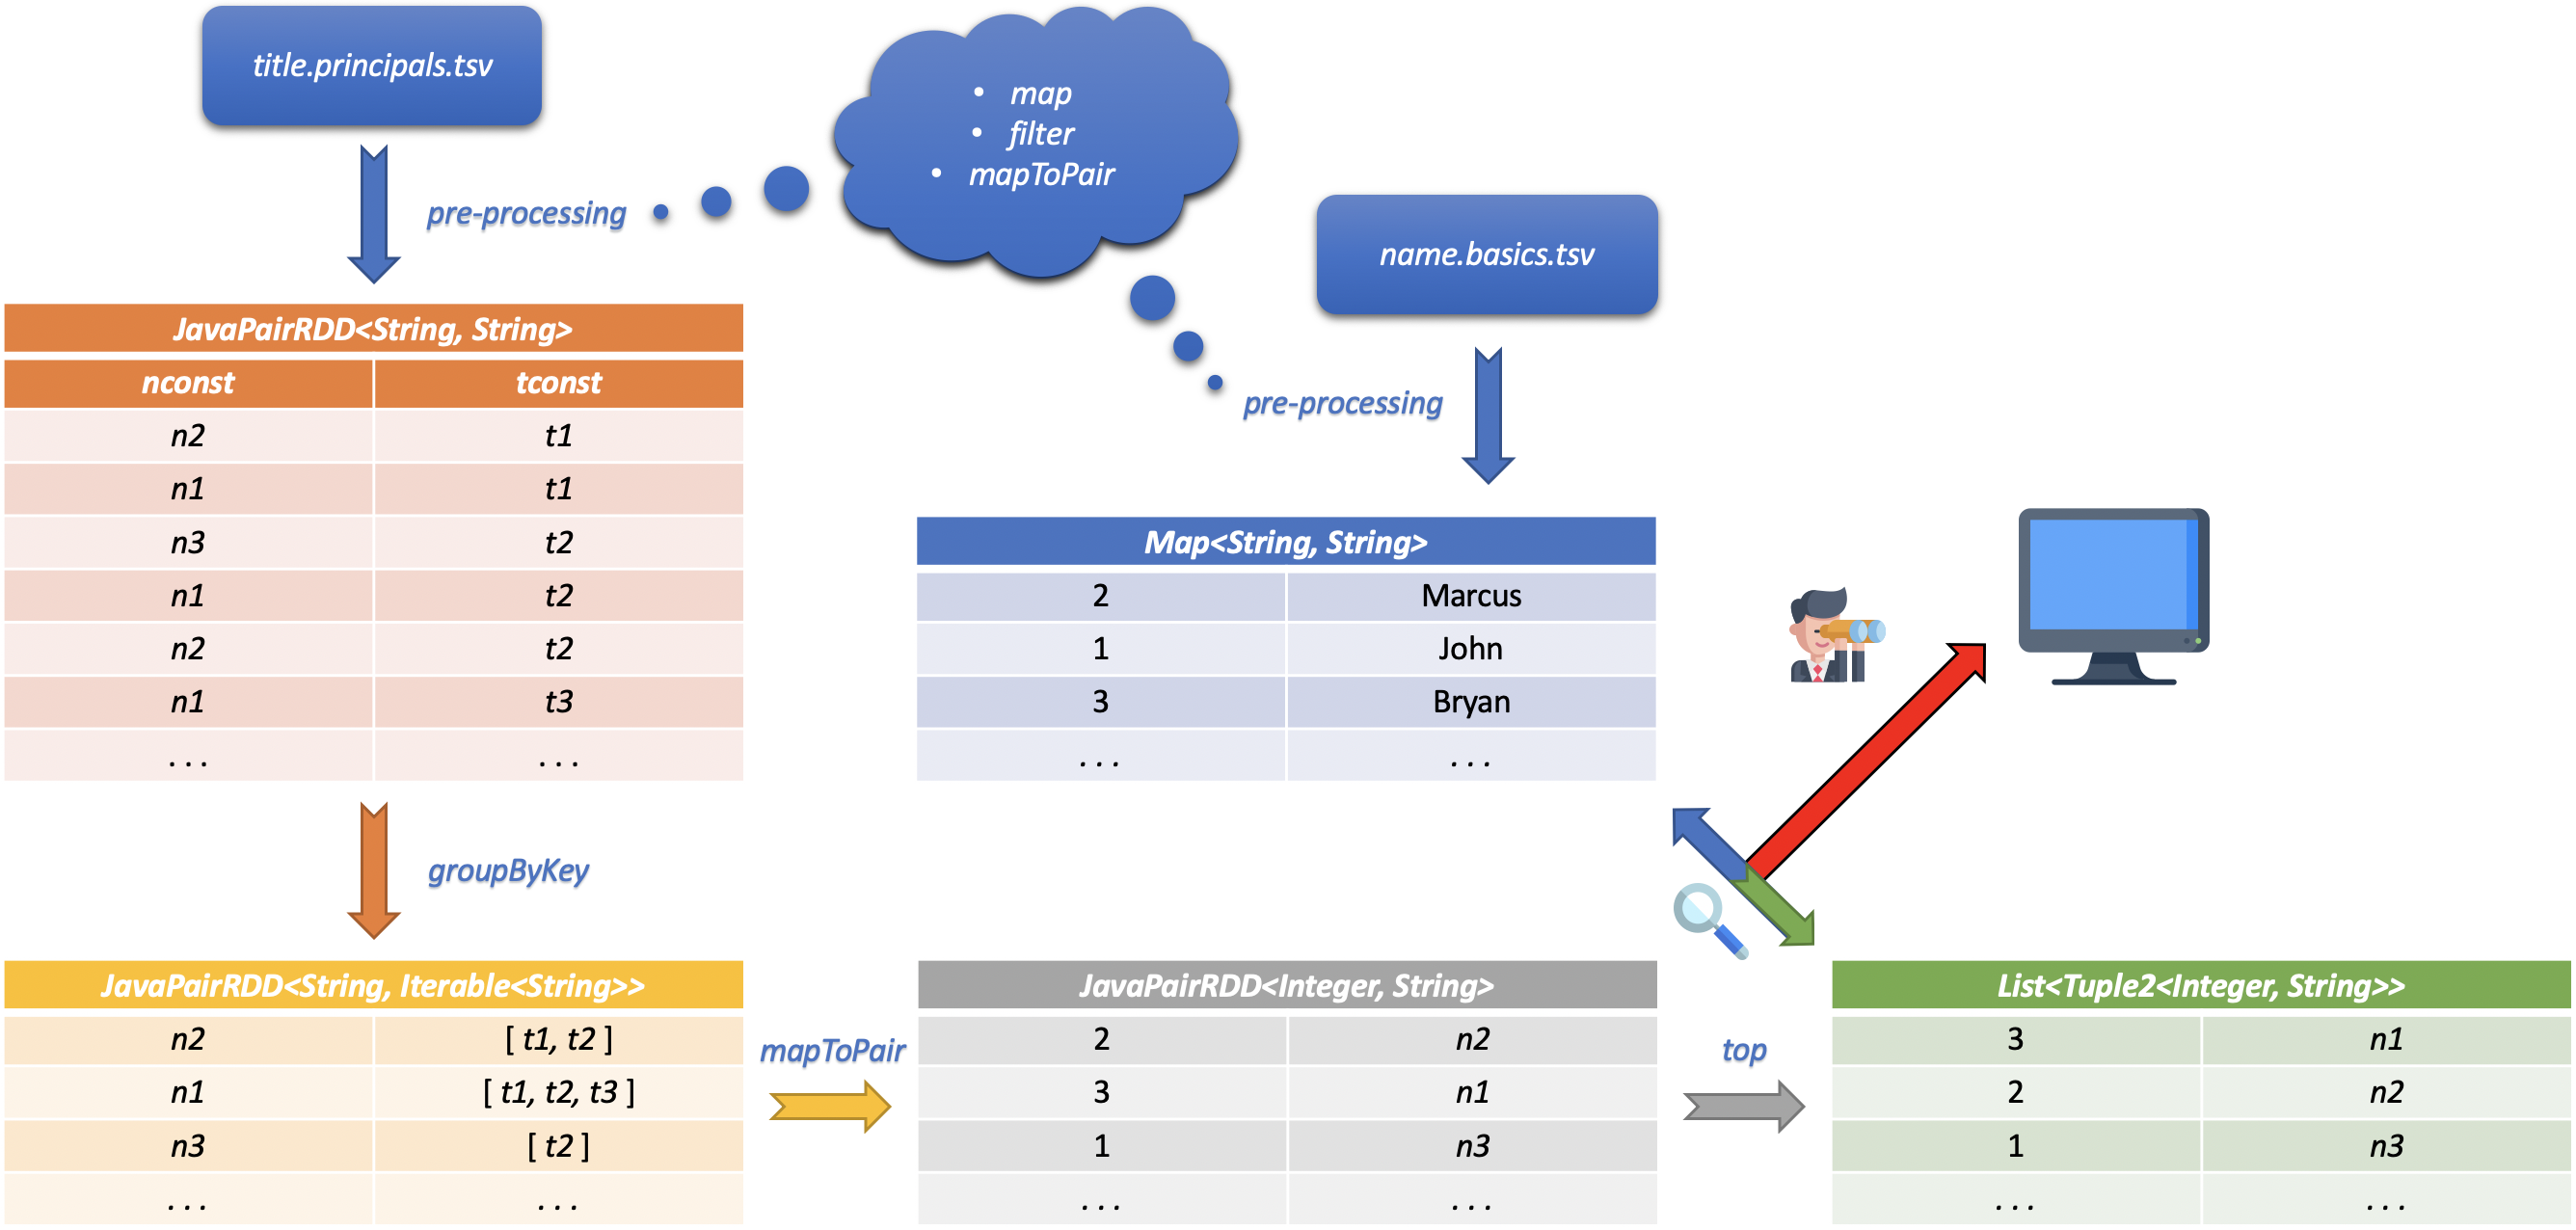
\includegraphics[width=1.0\textwidth]{Imagens/2ª Tarefa - Top10.png}
            \caption{2ª Tarefa (\textit{batch}) - Esquema do processamento relativo à subtarefa \textit{Top10}}
            \label{fig:1}
        \end{figure}

		\subsubsection{Alternativa} \label{sssec:Task2-Top10-Alternativa}
			Uma forma alternativa de resolver este exercício seria, na última fase do processamento, utilizar o método \textit{take} em detrimento da função \textit{top}.
			Esta escolha não foi tomada em consideração na implementação uma vez que o primeiro método necessita previamente que a informação esteja devidamente ordenada.
			Esta ordenação teria de ser realizada com a invocação do método \textit{sortByKey(false)}, colocando a contagem dos filmes em que cada ator participou de forma decrescente.
			Este último facto representa uma ineficiência no cálculo do resultado pretendido uma vez que é efetuada a ordenação completa da informação em causa e, para além disso, realiza-se desnecessariamente um passo computacional extra.

	\subsection{\textit{Friends}} \label{subsec:Task2-Friends}
		Neste exercício é requerido a computação do conjunto de colaboradores associado a cada ator, ou seja, o grupo dos atores que particapam nos mesmos filmes.
			
		Durante o processamento inicial do ficheiro \textsl{"title.principals.tsv"} é, tal como seria de esperar, ignorado o respetivo cabeçalho.
		Posteriormente, é extraída, linha após linha, a informação pertinente do mesmo, isto é, os identificadores do filme e do ator em questão, agrupando os dados pela primeira componente. Esta última ação é efetuada com recurso à chamada do método \textit{groupByKey}.
		De forma a obter o resultado solicitado nesta subtarefa, é necessário, nesta fase da computação, proceder à realização de uma operação denominada por produto cartesiano. Nesta operação computa-se, num dado momento, vários pares de atores que coloboraram num determinado filme.
		Uma vez realizado este cálculo, é invocado novamente o método \textit{groupByKey} de forma a obter o resultado pretendido, isto é, o conjunto de colaboradores para cada ator presente nos dados públicos do \textit{IMDb}.

		\begin{figure}[H]
            \centering
            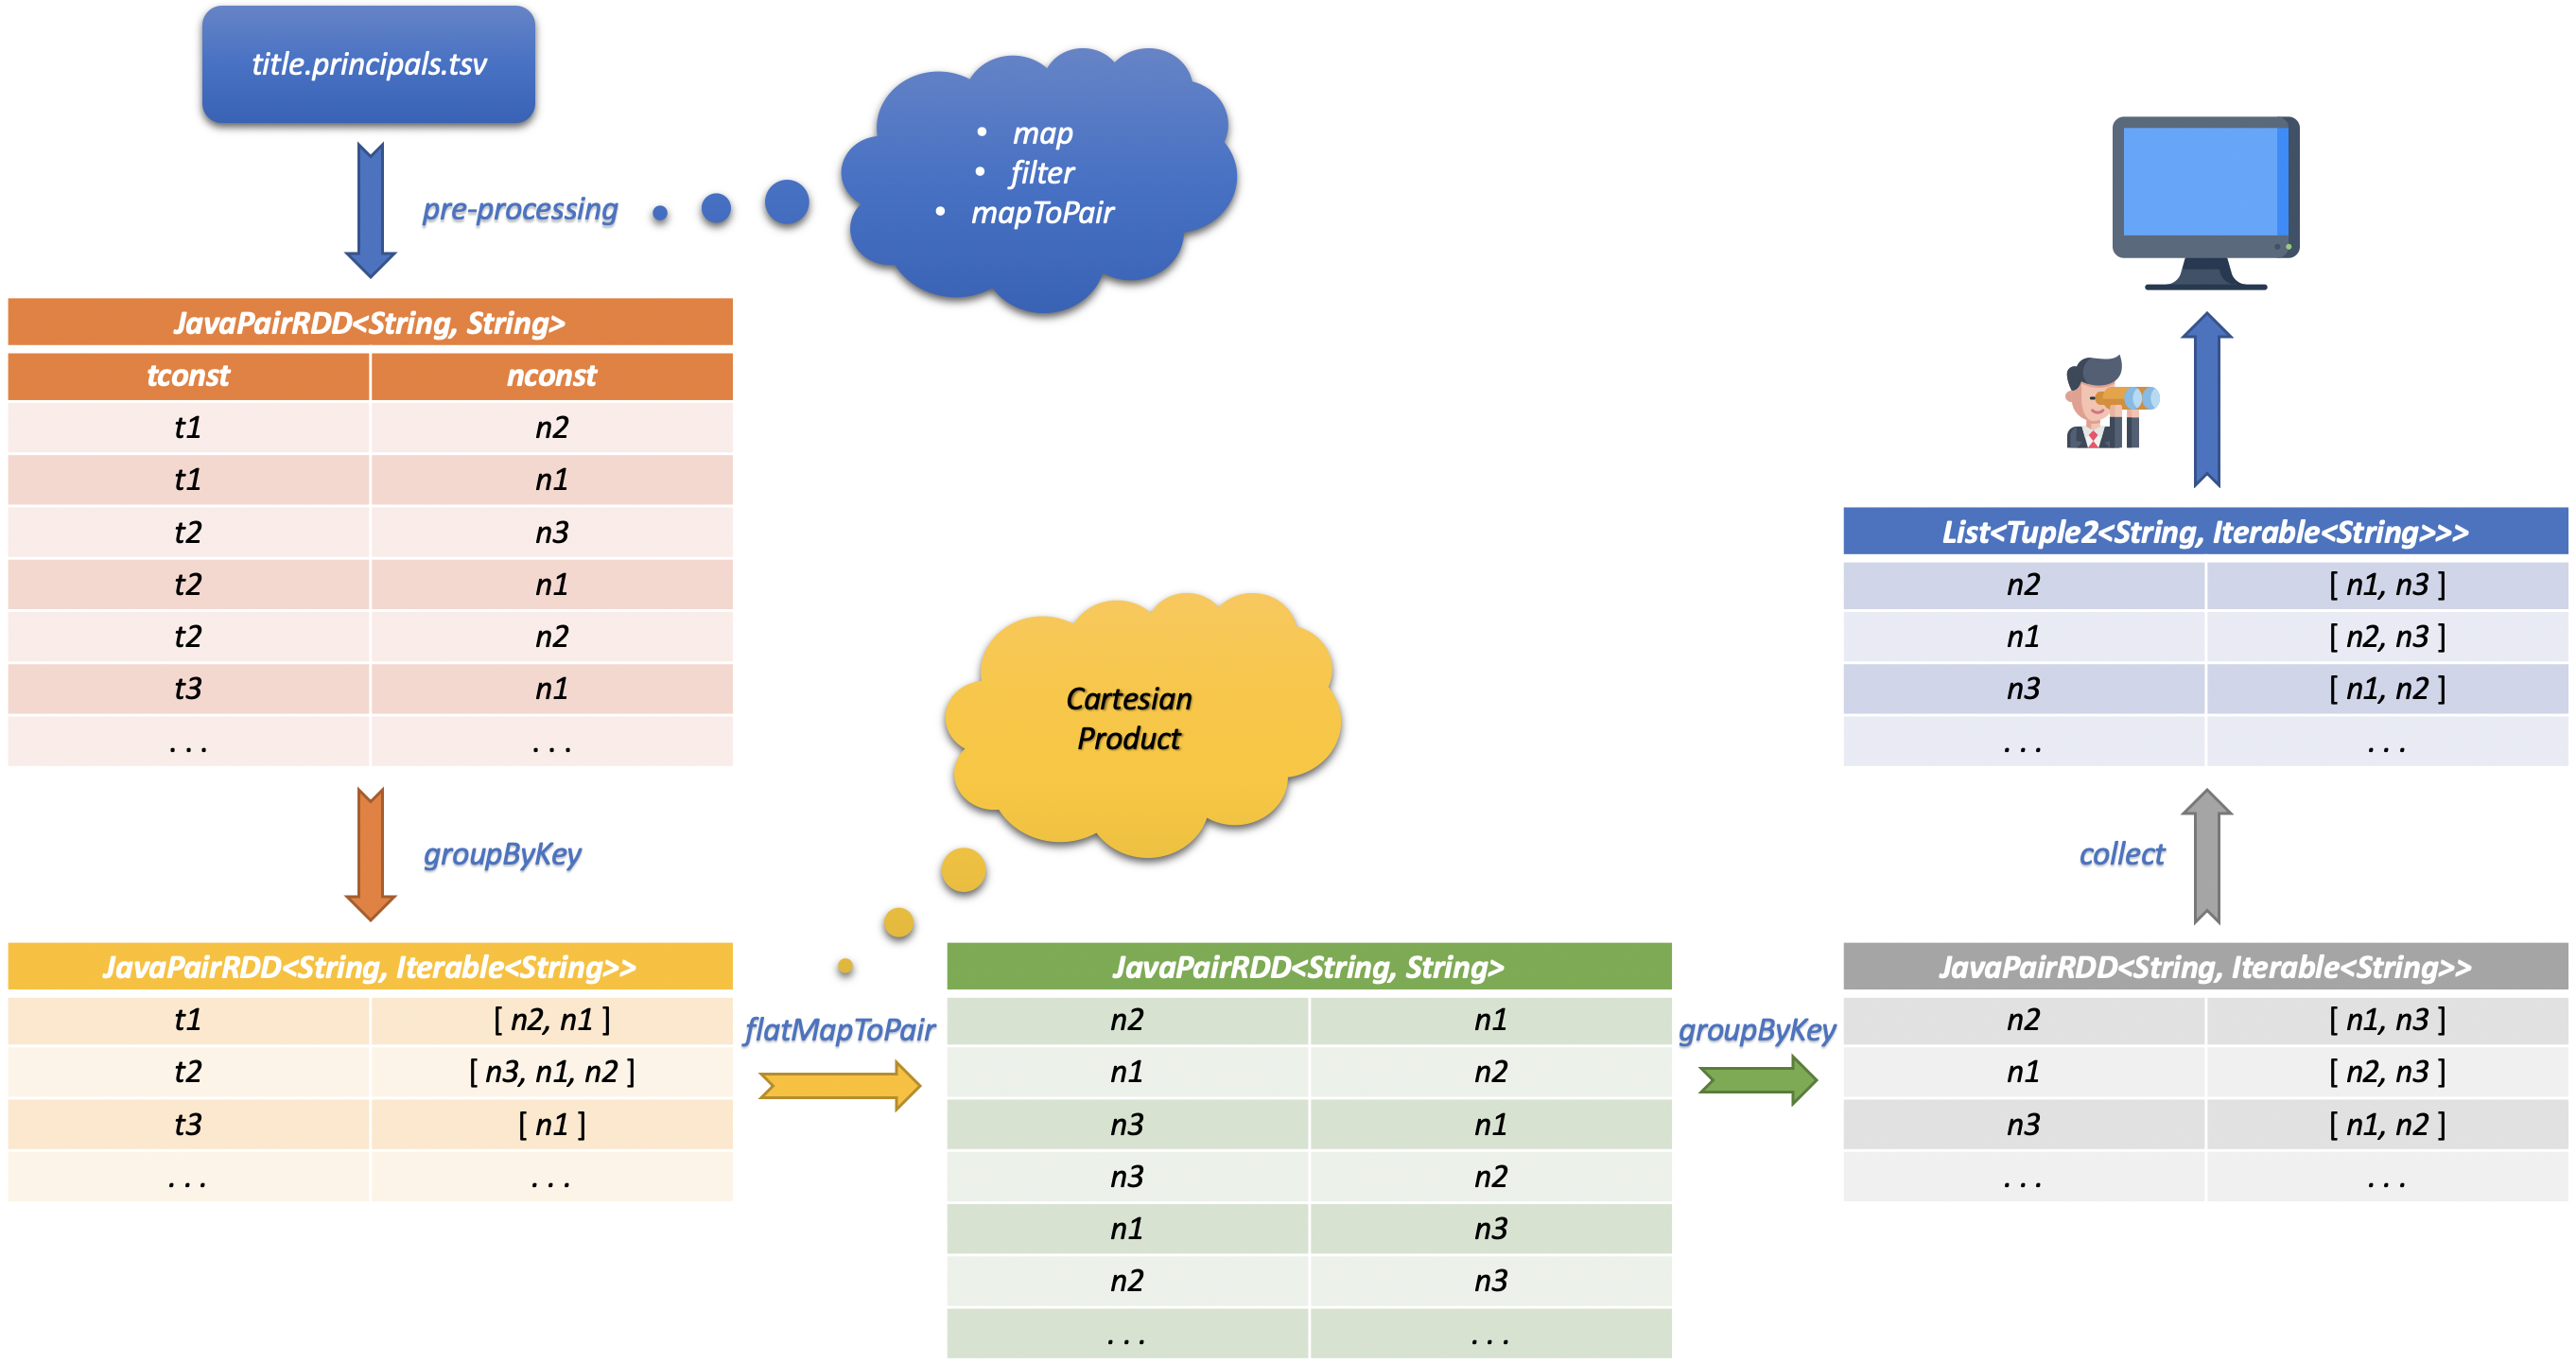
\includegraphics[width=1.0\textwidth]{Imagens/2ª Tarefa - Friends.png}
            \caption{2ª Tarefa (\textit{batch}) - Esquema do processamento relativo à subtarefa \textit{Friends}}
            \label{fig:2}
        \end{figure}

		\subsubsection{Alternativa} \label{sssec:Task2-Friends-Alternativa}

	\subsection{\textit{Ratings}} \label{subsec:Task2-Ratings}
		\subsubsection{Alternativa} \label{sssec:Task2-Ratings-Alternativa}

	\section{3ª Tarefa} \label{sec:Task3}


\chapter{Conclusão} \label{ch:Conclusion}
\large{
	
}

\appendix
\chapter{Observações} \label{ch:Observations}
\begin{itemize}
    \item Documentação \textit{Java} 8:
    \par \textit{\url{https://docs.oracle.com/javase/8/docs/api/}}
	\item \textit{Maven}:
	\par \textit{\url{https://maven.apache.org/}}
	\item \textit{Apache Spark}:
	\par \textit{\url{https://spark.apache.org/}}
	\item \textit{Docker}:
	\par \textit{\url{https://www.docker.com/}}
\end{itemize}

\end{document}